%---------------------------------------------------------------------------------------------------------------------------
% Kopf des Vortrags
%---------------------------------------------------------------------------------------------------------------------------

\part{Induktive Sensoren}
\begin{center}
Ulf Schmelzer (ulscit01@hs-esslingen.de) \\
Antonio Parrotta (anpait00@hs-esslingen.de)\\[1cm]
26. Oktober 2015 \\[1cm]
\end{center}


%---------------------------------------------------------------------------------------------------------------------------
% Textteil
%---------------------------------------------------------------------------------------------------------------------------
\section*{Einf�hrung}
%\label{Kap_Einf�hrung}

Induktive Sensoren werden in der Industrie eingesetzt, um ferromagnetische Materialien zu detektieren. Dieser Bericht befasst sich mit dessen Entstehung, Funktionsweise, dem Einsatzgebiet und dessen Eigenschaften.

%%%%%%%%%%%%%%%%%%%%%%%%%%%%%%%%%%%%%%%%%%%%%%%%%%%%%%%%%%%%%%%%%%%%%%%%%%%%%%%

\section*{Geschichte}
\label{geschichte}

Die Firma BASF beauftragte im Jahre 1958 das Unternehmen �Pepperl und Fuchs� in Mannheim, eine Alternative zu den bisher eingesetzten mechanischen Schaltern in der Automatisierung zu entwickeln. Die Vorgabe war, dass die Neuentwicklung mehrere tausende Schaltvorg�nge im chemischen Umfeld �berstehen muss, im Gegensatz zu den mechanischen Schaltern, die durch die Gase und Mittel schnell verschlissen.

Zu Beginn der Entwicklung wurden Bipolar-Transistoren verwendet, welche eine einfache Auswertung von
Schwingkreisen und Umwandlung in Schaltsignale erm�glicht haben. Durch den schnellen Wachstum im
Maschinenbau konnte parallel auch der induktive Sensor weiterentwickelt werden. Im Jahre 1968
entstand eine induktive Ausf�hrung des Rollenhebel-Endschalters nach DIN 43 694. Dieser hatte f�nf
verschiedene Seiten f�r die Sensorfl�che, damit alle m�glichen Anfahrrichtungen des mechanischen
Pendant nachempfunden werden konnten. Mittlerweile haben die induktiven N�herungsschalter
gr��tenteils die mechanischen Schalter abgel�st.\cite{geschichte}

%%%%%%%%%%%%%%%%%%%%%%%%%%%%%%%%%%%%%%%%%%%%%%%%%%%%%%%%%%%%%%%%%%%%%%%%%%%%%%%
\section*{Funktionsweise}
\label{funktionsweise}

Mit Hilfe eines LC-Schwingkreises wird eine elektromagnetisches Wechselfeld mit einer Frequenz zwischen 100kHz und 1MHz erzeugt. Durch den Einsatz eines hoch permeables Ferritmaterial kann dem entstehenden Magnetfeld in der Spule eine Vorzugsrichtung gegeben werden. Mit Hilfe eines Ferritkern kann das Feld auf den zu �berwachenden Bereich des Sensors abgestimmt werden.

Wird nun in das Erzeuge und gerichtet Magnetfeld das so genannte "Target" (das zu erkennende Ziel) eingebracht wird nach dem Induktionsgesetz wie bei einem Transformator dem Schwingkreis Energie entzogen. Siehe Abbildung <Ersatzschaltbild mit Transformator>
Dabei kann die Spule des LC-Schwingkreises als Prim�rwicklung und das "Target" als Sekund�rwicklung mit Widerstand als Verbraucher dargestellt werden.

Die nun auftretenden Wirbelstromverluste sind von mehreren Faktoren abh�ngig.

- Abstand und der Lage des Gegenstandes vor dem N�herungsschalter 
- Abmessungen des Gegenstandes und seiner �u�eren Form 
- elektrische Leitf�higkeit und seiner Permeabilit�t. <quelle pdf doc>

Das nun entstehende ged�mpfte Signal kann mit Hilfe eines Operationsverst�rkers ausgewertet werden um ein Bin�res Signal zu erzeugen. In der Realit�t wird das Signal meistens noch weiter ausgewertet um z.b. flattern, wenn sich ein Gegenstand sehr langsam n�hert, oder ein fehlerhaftes schalten beim anlegen der Betriebsspannung und w�hrend des ein schwingen des LC-Schwingkreises zu verhindern.



\newpage
\begin{figure}[h]
	\centering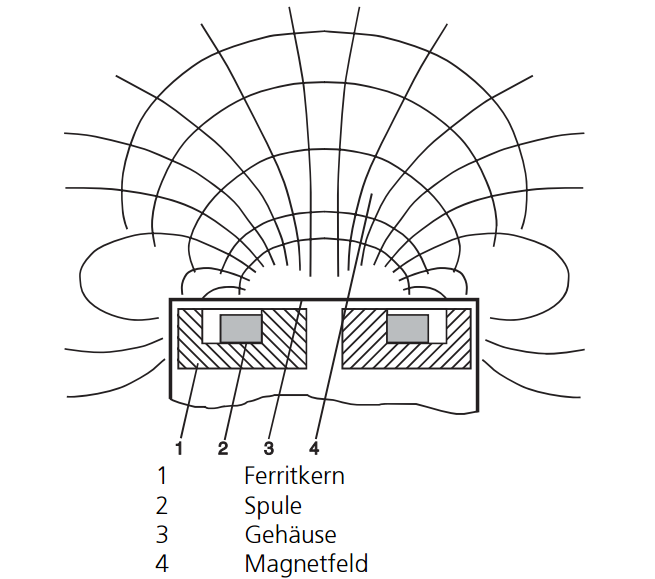
\includegraphics[width=.4\textwidth]{induktiv_sensoren/magnetfeld_sensor.png}
	\caption{Magnetfeld eines induktiven Sensors\cite{ifm}}
	\label{fig:magnetfeld}
\end{figure}


%%%%%%%%%%%%%%%%%%%%%%%%%%%%%%%%%%%%%%%%%%%%%%%%%%%%%%%%%%%%%%%%%%%%%%%%%%%%%%%
%------------------------------------------------------------------------------------------------------------------------
\section*{Analog Sensor}
\label{analogsensor}
Bei Analogen Sensoren wird das entstehende Signal ausgewertet und z.b. mit Hilfe eines Micocontrollers vorverarbeitet oder als Analogwert im Bereich von 4-20mA zur�ckgeliefert. Dieses Signal kann z.b. zur Abstandsmessung genutzt werden. Dabei muss allerdings darauf geachtet werden das sich das n�hernde Objekt immer auf der selben bahn und Winkel befindet und auch das Material immer das selbe ist da diese Parameter alle in die Wirbelstromverluste einflie�en da es sonst zu stark variierenden Messergebnissen kommen kann.
Aufgrund dieser Problematik werden Induktivsensoren eher selten zur Abstandsmessung eingesetzt.

%------------------------------------------------------------------------------------------------------------------------
\section*{Fazit}
%\label{Kap_Fazit}

Meines Erachtens sind diese Tests unerl�sslich f�r ein zuverl�ssiges Produkt. Denn durch die Vielzahl an Phasen werden pro Phase mehr und mehr Fehler erkannt und behoben. Es f�ngt an mit gravierenden Fehlern wie abst�rzen des Produkts bis hin zu Feinheiten wie Textur Makeln. Das alles ist wichtig damit die Software sp�ter stabil l�uft und es nicht zu Problemen kommt. Ein anderer wichtiger Punkt ist die Werbung die dadurch erzielt wird, denn durch das Testen der Software wird das Interesse geweckt und die Nachfrage kann dadurch sehr steigen.

%%%%%%%%%%%%%%%%%%%%%%%%%%%%%%%%%%%%%%%%%%%%%%%%%%%%%%%%%%%%%%%%%%%%%%%%%%%%%%%
\newpage
\begin{thebibliography}{}
%\addcontentsline{toc}{section}{Literatur}
\bibitem{geschichte}
Process.Vogel:\textit{"'Vergangenheit und Zukunft des induktiven N�herungsschalters"'},\\
\href{http://www.process.vogel.de/automatisierung_prozessleittechnik/articles/145538/}{http://www.process.vogel.de/automatisierung\\\_prozessleittechnik/articles/145538/}, \\Aufrufdatum: 30.09.2015

\bibitem{ifm}
IFM:\textit{"'Schulungsunterlagen Induktive Sensoren"'}, \href{http://www.seo-analyse.com/seo-lexikon/e/entwicklungsstadium}{http://www.ifm.com/obj/S100d.pdf},\\
Aufrufdatum: 30.09.2015

\bibitem{Ref_foerder}
F�rderland:\textit{"'Entwicklungsstadien von Software"'},\\
\href{http://www.foerderland.de/itoffice/it/it-entwicklung/entwicklungsstadien-von-software/}{http://www.foerderland.de/itoffice/it/it-entwicklung/\\entwicklungsstadien-von-software/}, \\
Aufrufdatum: 01.11.2014

\bibitem{Ref_wikipedia14}
Wikipedia:\textit{"'Entwicklungsstadium: Beta-Version"'},\\
\href{http://de.wikipedia.org/wiki/Entwicklungsstadium\_\%28Software\%29}{http://de.wikipedia.org/wiki/\\Entwicklungsstadium\_\%28Software\%29}, \\
Aufrufdatum: 01.11.2014

\bibitem{Ref_centercode11}
Centercode:\textit{"'alpha-vs-beta-testing"'}, \href{http://www.centercode.com/blog/2011/01/alpha-vs-beta-testing/}{http://www.\\centercode.com/blog/2011/01/alpha-vs-beta-testing/}, \\
Aufrufdatum: 01.11.2014

\end{thebibliography}
%%%%%%%%%%%%%%%%%%%%%%%%%%%%%%%%%%%%%%%%%%%%%%%%%%%%%%%%%%%%%%%%%%%%%%%%%%%%%%%
